% F1 — Harness anatomy: the five runtime jobs with the components WE have under each.
% Solid = DEPLOYED on disk at the census date (2026-09-02); dashed = PROPOSED (register row or law file only).
% COLOUR GRAMMAR (PI, 2026-09-03, after Schüssler+2026 arXiv:2608.23270 Fig. 1 — design reference, not cited):
%   blue = deterministic code; green = model-judgement role (agent); white/grey frame = documents & records;
%   amber = the human; dashed = PROPOSED; hatched enclosures = the two harness layers (outer grey = hosted product,
%   inner green = the repository layer). Same grammar in F2/F4/F5. Tie-break (gate 2026-09-03): a document the
%   model reads (protocol, guide, contract, memory) is WHITE; green is reserved for a ROLE the model plays.
% Standalone: pdflatex fig_F1_harness_anatomy.tex -> PDF; rasterize for the figure-verifier.
% Every component name here appears as a row of T1 (paper_agentic/T1_component_roster_DRAFT.md).
% STYLE PASS (PI 2026-09-03, decision 26, after Yang+2026 arXiv:2607.08938 Figs. 1-3 as design reference): Source Sans Pro,
% softer corners, 1 pt soft-grey arrows with round caps/joins, light frames on neutral boxes; texts and the D24 colour grammar unchanged.
\documentclass[tikz,border=4pt]{standalone}
\usepackage[T1]{fontenc}
\usepackage[default]{sourcesanspro}
\usetikzlibrary{positioning,fit,calc,shapes.geometric,arrows.meta,backgrounds,patterns}
\newcommand{\nohyph}{\hyphenpenalty=10000 \exhyphenpenalty=10000 }
\definecolor{codefill}{RGB}{199,217,239}\definecolor{codeline}{RGB}{59,110,165}
\definecolor{agentfill}{RGB}{226,240,217}\definecolor{agentline}{RGB}{58,125,52}
\definecolor{humanfill}{RGB}{253,236,200}\definecolor{humanline}{RGB}{191,124,0}
\definecolor{docline}{RGB}{110,110,110}
\begin{document}
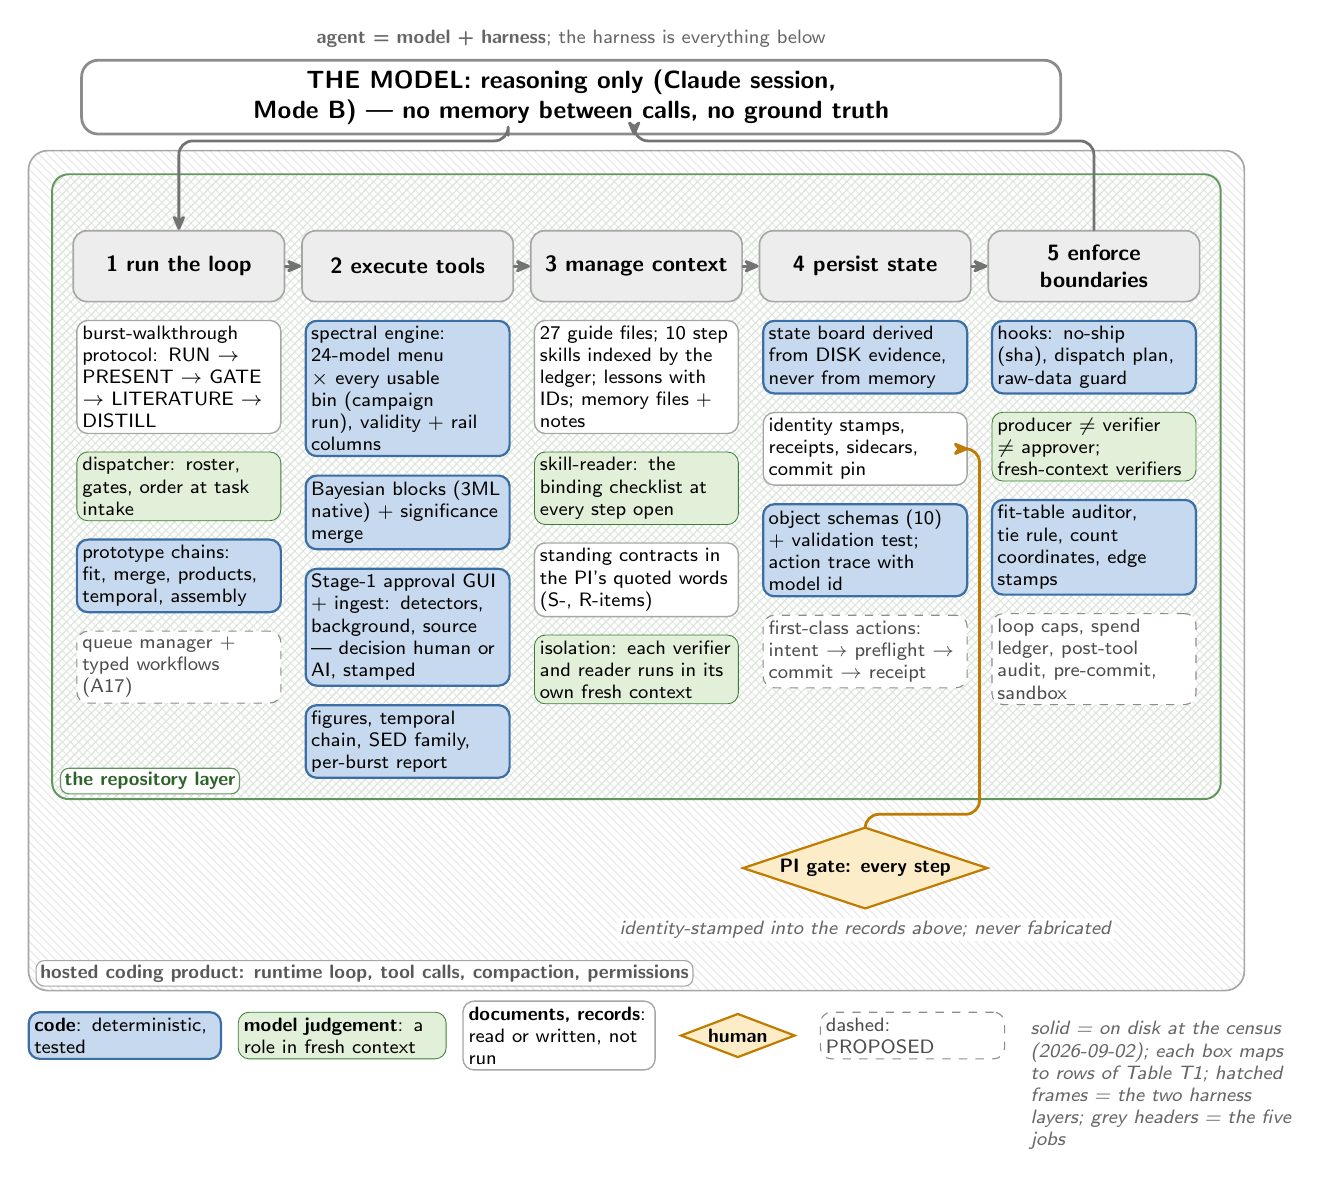
\begin{tikzpicture}[
  font=\sffamily\footnotesize, node distance=2.2mm and 2mm,
  job/.style={draw=black!35, line width=0.6pt, rounded corners=5pt, fill=black!7, text width=24.5mm, align=center, minimum height=9mm, font=\sffamily\bfseries\footnotesize},
  box/.style={draw, rounded corners=4pt, text width=24.5mm, align=left, inner sep=2pt, font=\sffamily\scriptsize, execute at begin node=\nohyph},
  code/.style={box, fill=codefill, draw=codeline, line width=0.8pt},
  agent/.style={box, fill=agentfill, draw=agentline, line width=0.3pt},
  doc/.style={box, fill=white, draw=black!35, line width=0.5pt},
  prop/.style={box, dashed, fill=white, draw=black!45, text=black!70},
  model/.style={draw=black!45, line width=1pt, rounded corners=6pt, fill=white, text width=122mm, align=center, minimum height=9mm, font=\sffamily\bfseries\small},
  human/.style={draw=humanline, thick, diamond, aspect=3, fill=humanfill, inner sep=1pt, font=\sffamily\scriptsize\bfseries},
  arr/.style={-{Stealth[length=2.4mm,width=2mm,round]}, line width=1pt, black!55, rounded corners=5pt, line cap=round, line join=round},
  lab/.style={font=\sffamily\scriptsize\itshape, text=black!60}]

% the model, and the loop around it
\node[model] (model) {THE MODEL: reasoning only (Claude session, Mode~B) --- no memory between calls, no ground truth};
\node[lab, above=1mm of model, font=\sffamily\scriptsize, fill=white, inner sep=1pt] (toplab) {\textbf{agent = model + harness}; the harness is everything below};

% five jobs
\node[job, below=12mm of model.south west, anchor=north west, xshift=-1mm] (loop) {1 run the loop};
\node[job, right=of loop] (tools) {2 execute tools};
\node[job, right=of tools] (ctx) {3 manage context};
\node[job, right=of ctx] (state) {4 persist state};
\node[job, right=of state] (bound) {5 enforce boundaries};

% components under each job (colour = what executes; dashed = PROPOSED)
\node[doc, below=of loop] (l1) {burst-walkthrough protocol: RUN $\to$ PRESENT $\to$ GATE $\to$ LITERATURE $\to$ DISTILL};
\node[agent, below=of l1] (l2) {dispatcher: roster, gates, order at task intake};
\node[code, below=of l2] (l3) {prototype chains: fit, merge, products, temporal, assembly};
\node[prop, below=of l3] (l4) {queue manager + typed workflows (A17)};

\node[code, below=of tools] (t1) {spectral engine: 24-model menu $\times$ every usable bin (campaign run), validity + rail columns};
\node[code, below=of t1] (t2) {Bayesian blocks (3ML native) + significance merge};
\node[code, below=of t2] (t3) {Stage-1 approval GUI + ingest: detectors, background, source --- decision human or AI, stamped};
\node[code, below=of t3] (t4) {figures, temporal chain, SED family, per-burst report};

\node[doc, below=of ctx] (c1) {27 guide files; 10 step skills indexed by the ledger; lessons with IDs; memory files + notes};
\node[agent, below=of c1] (c2) {skill-reader: the binding checklist at every step open};
\node[doc, below=of c2] (c3) {standing contracts in the PI's quoted words (S-, R-items)};
\node[agent, below=of c3] (c4) {isolation: each verifier and reader runs in its own fresh context};

\node[code, below=of state] (s1) {state board derived from DISK evidence, never from memory};
\node[doc, below=of s1] (s2) {identity stamps, receipts, sidecars, commit pin};
\node[code, below=of s2] (s3) {object schemas (10) + validation test; action trace with model id};
\node[prop, below=of s3] (s4) {first-class actions: intent $\to$ preflight $\to$ commit $\to$ receipt};

\node[code, below=of bound] (b1) {hooks: no-ship (sha), dispatch plan, raw-data guard};
\node[agent, below=of b1] (b2) {producer $\neq$ verifier $\neq$ approver; fresh-context verifiers};
\node[code, below=of b2] (b3) {fit-table auditor, tie rule, count coordinates, edge stamps};
\node[prop, below=of b3] (b4) {loop caps, spend ledger, post-tool audit, \mbox{pre-commit}, sandbox};

% the human gate
\coordinate (pianchor) at (s4.south |- t4.south);
\node[human, below=6mm of pianchor, anchor=north] (pi) {PI gate: every step};


% arrows: loop
\draw[arr] ($(model.south)+(-8mm,0)$) -- ++(0,-0.7mm) -| (loop.north);
\draw[arr] (loop.east) -- (tools.west);
\draw[arr] (tools.east) -- (ctx.west);
\draw[arr] (ctx.east) -- (state.west);
\draw[arr] (state.east) -- (bound.west);
\draw[arr] (bound.north) |- ($(model.south)+(8mm,-0.7mm)$) -- ($(model.south)+(8mm,0)$);
\draw[arr, humanline] (pi.north) -- ++(0,1.5mm) -| ($(s4.east)+(1.5mm,0)$) |- (s2.east);
\node[lab, below=1mm of pi, fill=white, inner sep=1pt] (pilab) {identity-stamped into the records above; never fabricated};

% the two harness layers (drawn behind): outer grey hatch = the hosted product; inner green frame painted OVER it
\begin{scope}[on background layer]
  \coordinate (headroom) at ($(loop.north)+(0,4.5mm)$);
  \node[inner sep=2.5mm, fit=(headroom)(loop)(bound)(l4)(b4)(t1)(t4)] (repo) {};
  \coordinate (footroom) at ($(pilab.south)+(0,-3.2mm)$);
  \node[draw=black!35, line width=0.6pt, rounded corners=7pt, pattern=north west lines, pattern color=black!9, inner sep=3mm,
        fit=(repo)(pi)(pilab)(footroom)] (host) {};
  \node[draw=agentline!80, line width=0.7pt, rounded corners=6pt, pattern=north east lines, pattern color=agentline!20, inner sep=0, fit=(repo)] {};
  \node[fill=white, draw=black!35, rounded corners=3pt, inner sep=1.5pt, font=\sffamily\scriptsize\bfseries, text=black!65,
        anchor=south west] at ($(host.south west)+(1mm,0.6mm)$) {hosted coding product: runtime loop, tool calls, compaction, permissions};
  \node[fill=white, draw=agentline!80, rounded corners=3pt, inner sep=1.5pt, font=\sffamily\scriptsize\bfseries, text=agentline!80!black,
        anchor=south west] at ($(repo.south west)+(1mm,0.6mm)$) {the repository layer};
\end{scope}

% legend row (below the outer enclosure)
\node[code, anchor=north west, text width=23mm] (leg1) at ($(host.south west)+(0,-2.5mm)$) {\textbf{code}: deterministic, tested};
\node[agent, right=2mm of leg1, text width=25mm] (leg2) {\textbf{model judgement}: a role in fresh context};
\node[doc, right=2mm of leg2, text width=23mm] (leg3) {\textbf{documents, records}: read or written, not run};
\node[human, right=3mm of leg3, aspect=2.6] (leg4) {human};
\node[prop, right=3mm of leg4, text width=22mm] (leg5) {dashed: PROPOSED};
\node[lab, anchor=north west, text width=34mm, align=left, execute at begin node=\nohyph] at ($(leg5.north east)+(2mm,0)$) {solid = on disk at the census (2026-09-02); each box maps to rows of Table~T1; hatched frames = the two harness layers; grey headers = the five jobs};
\end{tikzpicture}
\end{document}
